\documentclass[a4j,12pt]{jarticle}
\usepackage{booktabs}
\usepackage[dvipdfmx]{graphicx}
\usepackage{listings,jlisting}
\title{JPF を適用可能な Java プログラムの構成法 \\ に関する実験と考察}
\author{北陸先端科学技術大学院大学 情報科学研究科 \\ 加藤 裕\thanks{学籍番号 1110020, E-mail: y-kato@jaist.ac.jp}}
\和暦
\date{平成24年1月30日}
\begin{document}
\maketitle

\newpage
\setcounter{tocdepth}{3}
\tableofcontents
\section{背景}

近年,情報化社会が大きく発展する中で,ソフトウェアの役割は極めて大きくなっている.利用者の拡大や多様化するニーズなどに対応するため,ソフトウェアは大規模複雑化を続けており,限られた時間の中でいかに不具合のないソフトウェアを開発するかが重要視されている.

そうした中で,ソフトウェアが仕様通りに実装されているかを効率よく調べる検証技術が注目されている.大規模複雑化するソフトウェアを手作業で検証するには限界があるからである.

ソフトウェアの正しさを効率よく検証するための方式として,モデル検査と呼ばれる手法が挙げられる.モデル検査は,プログラムを解析し ``状態''を抽出,それを木構造にマッピングし全ての状態の探索を行い,仕様を満たしているかを判別する技術である.本レポートで取り上げる JPF  (Java PathFinder) \cite{JPF} は,Java \footnote{Javaは,Oracle Corporation 及びその子会社,関連会社の米国及びその他の国における登録商標.} で記述されたプログラムを対象としたモデル検査器で,表明違反,キャッチされない例外,デッドロック,データ競合といった諸問題を全ての実行パスの中から見つけ出す事ができる.そして Java は,世の中で最も利用されているプログラミング言語であり \cite{TIOBE},ネットワーク,ビジネス,そして組み込みといった幅広い分野に普及しているため,こうしたソフトウェアへモデル検査を容易に適用できれば,高信頼化実現に向けて多いに助けになると考えられる.

しかし JPF は,その動作原理ゆえに様々な制約があり,ネットワークやデータベース入出力,GUI などといった様々な種類の処理が組合わさった一般的なアプリケーションに対してそのまま適用することは難しい.そこで本レポートでは,JPF の持つ機能と特徴について調査した上で,ネットワークアプリケーションを例にとり,JPF を適用するにあたって直面する様々な問題を解決し構成する方法を実験により明らかにし,JPF の有用性について考察する.

\section{JPF の機能と特徴}

\subsection{JPF とは何か}

JPF のウェブサイトでは,JPF を表す一言として次のように書かれている: \cite{JPF}

\begin{quotation}
``JPF is an explicit state software model checker for Java\texttrademark  bytecode''
\end{quotation}

つまり JPF は,Java バイトコードのための明示的な状態モデル検査を行うツールである.Java バイトコードは,Java 仮想マシン上で実行可能な中間コードを指す.JPF は,自らが持つ仮想マシン上でJava プログラムを実行しながらモデル検査を行うことができる.

JPF は,NASA (米国航空宇宙局) の研究者が中心となって開発された.また,ソースコードは NOSA (NASA Open Source Agreement) ライセンスの下に公開されており,誰でもコードを閲覧したり,改変して利用することができる.また,拡張可能な構造になっており,様々な拡張がサブプロジェクトとして開発されている.

\subsection{JPF の動作原理}

JPF は,プログラムのヒープやスレッド・スタックなどから ``状態'' を抽出し,それらを木構造にマッピングし,探索を行う.

JPF が状態群を探索する様子を次の図 \ref{figure:states-mc} に示す.

\begin{figure}[here]
\centering
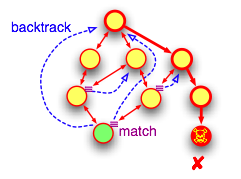
\includegraphics[width=7cm]{images/states-mc.png}
\caption{モデル検査における状態の探索 \cite{JPF}}
\label{figure:states-mc}
\end{figure}

JPF は,状態と状態のマッチングを繰り返しながら探索を広げて行き,バックトラックを駆使して全ての実行パスを網羅するまで繰り返す.これにより,人手をかけずに高精度で不具合を発見することができる.

JPF の基本構成を以下の図 \ref{figure:jpf-basic} に示す.

\begin{figure}[here]
\centering
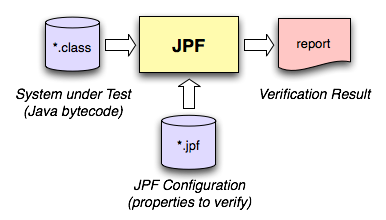
\includegraphics[width=9cm]{images/jpf-basic.png}
\caption{JPF の基本構成 \cite{JPF}}
\label{figure:jpf-basic}
\end{figure}

JPF は,入力に Java プログラムのバイトコード一式と,プロパティと呼ばれる様々な情報・パラメータを集めたファイルを与える.

プロパティには,クラスパスとメインクラス名のほか,プログラムの引数,レポートに表示したい項目,Listener の指定,その他様々なカスタマイズが可能になっている.

\subsection{JPF の主要機能}

\subsubsection{ハンドルされない例外・エラーの検出}

Java 言語には例外処理機構が備わっており,例外が発生する可能性が明記されている処理に対して,try-catch (-finally) 文でその場で例外処理を書くか, throws を使って呼出し元へ処理を任せるかを選択できる.もしどちらも行わない場合はコンパイラがエラーを出力し,記述漏れを阻止する仕組みになっている.

しかし RuntimeException (実行時例外) や,それを継承した IllegalArgumentException (不正引数例外), NullPointerException (null 参照例外), ArithmeticException (算術例外) などは,例外の対応を記述するは任意である.これは,開発の負担と信頼性とのバランスが,設計者や開発者に委ねられている事を意味する \cite{JavaTGP}.そして現実には,ハンドルされない RuntimeException 系の例外が多数残され,ソフトウェアの信頼性を損なう一要因になっている.

JPF を用いれば,こうしたハンドルされない RuntimeException 系の全ての例外や,AssertionError などのエラーを検出することができる.例えば,以下のように例外が仕込まれたプログラムがあったとする.

\begin{lstlisting}[label=src:ex-exception, caption=例外の検出,language=Java]
public class StopWatch {
    public static void main(String[] args) {
        long tStart = System.currentTimeMillis();
        System.out.println("some lengthy computation..");
        long tEnd = System.currentTimeMillis();
        if (tEnd - tStart > 1000) {
            throw new RuntimeException("it took too long..");
        }
        System.out.println("all fine, finished in time");
    }
}
\end{lstlisting}

4 行目にある標準出力の前後で時刻をミリ秒単位で計測しており,その差が 1000 ミリ秒 (1 秒) 以上あれば RuntimeException をスローするというものである.

標準出力 1 行実行するのに 1 秒もかかるようなエラーケースをテストするのは容易ではない.しかし JPF によるモデル検査は,可能性がある状態遷移は全て探索するので,こうしたケースも検出することができる.

上記プログラムに対する JPF のレポートを次に示す.

\begin{verbatim}
====================================================== system under test
application: StopWatch.java

====================================================== search started: ...
some lengthy computation..
all fine, finished in time
all fine, finished in time

====================================================== error #1
gov.nasa.jpf.jvm.NoUncaughtExceptionsProperty
java.lang.RuntimeException: it took too long..
	at StopWatch.main(StopWatch.java:31)


====================================================== snapshot #1
thread id=0,name=main,status=RUNNING,priority=5,lockCount=0,suspendCount=0
  call stack:
	at StopWatch.main(StopWatch.java:31)


====================================================== results
error #1: gov.nasa.jpf.jvm.NoUncaughtExceptionsProperty 
                  "java.lang.RuntimeException: it took too long..  at..."

====================================================== statistics
elapsed time:       00:00:00
states:             new=3, visited=1, backtracked=2, end=2
search:             maxDepth=2, constraints hit=0
choice generators:  thread=1 (signal=0, lock=1, shared ref=0), data=1
heap:               new=339, released=20, max live=319, gc-cycles=3
instructions:       2969
max memory:         81MB
loaded code:        classes=78, methods=971

====================================================== search finished: ...
\end{verbatim}

キャッチされない RuntimeException が検出された事が,error 欄,results 欄からわかる.

これらの結果から JPF がどのような探索を行っているかを想像したものを以下の図 \ref{figure:exception-search} に示す.

\begin{figure}[here]
\centering
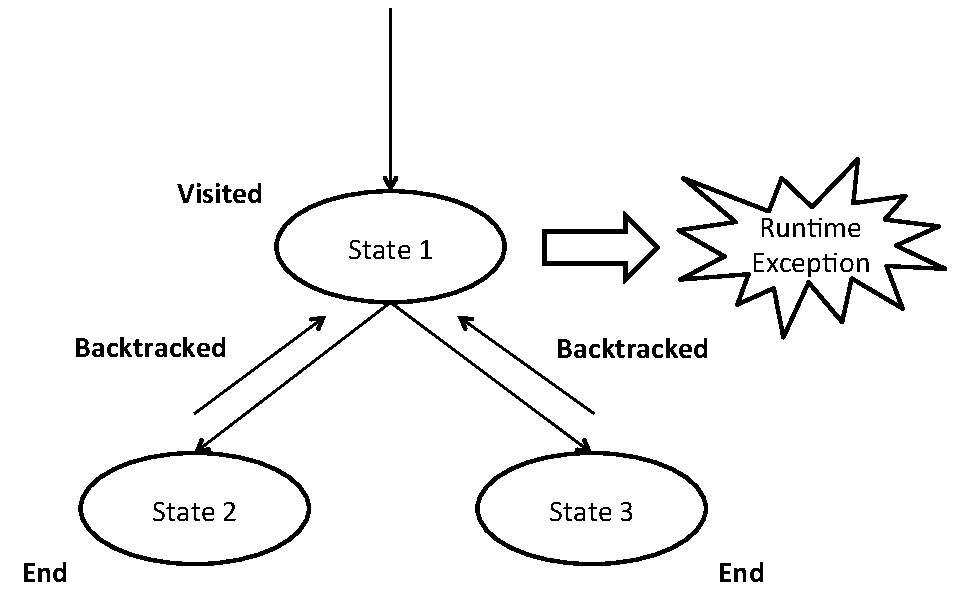
\includegraphics[width=12cm]{images/exception-search.pdf}
\caption{例外処理の探索の様子}
\label{figure:exception-search}
\end{figure}

探索中の出力や statistics 欄の end 状態数から,正常終了するパスが 2 つ存在することがわかった.またバックトラックを繰り返すことで,途中の状態から RuntimeException に至るパスを検出したことがわかった.

\subsubsection{デッドロック検出}

デッドロックは,複数のスレッド(プロセス)と複数のリソースがある場面で,いくつかの条件が重なるとプログラムが全く動かなくなってしまうという不具合である.デッドロックは,以下の 4 つの性質を全て満たした場合に成立する \cite{DBLP:journals/csur/CoffmanES71} \cite{MOS2}.

\begin{itemize}
\item 相互排除性: リソースは 1 度に 1 プロセスにのみ与えられる
\item 保有と待ち条件: プロセスは複数のリソースを要求できる
\item 横取りなし条件: 他のプロセスのリソースを奪うことができない
\item 循環待ち条件: リソース待ちプロセスの循環鎖がある
\end{itemize}

デッドロックを JPF が検出する様子を確かめるために,二つのスレッド th1, th2 と二つのリソース Resource A, Resource B を持ち,互いのスレッドが二つの資源の確保と解放を繰り返す(保有と待ち条件を満たす)プログラムを作成した.

なお,ロック機構には,Java に用意されている排他制御機構 (synchronized 文) を利用した.これは,デッドロック成立条件のうちの相互排除性と横取りなし条件を満たすことになる.つまり,この時点で残る成立条件は循環待ち条件のみとなる.

以下は,そのプログラムを JPF に掛けたときのレポートのエラー欄とスナップショット欄を抜き出したものである.

\begin{verbatim}
====================================================== error #1
gov.nasa.jpf.jvm.NotDeadlockedProperty
deadlock encountered:
  thread id=0,name=main,status=WAITING,priority=5,lockCount=0,suspend...
  thread id=1,name=Thread-1,status=BLOCKED,priority=5,lockCount=0,sus...
  thread id=2,name=Thread-2,status=BLOCKED,priority=5,lockCount=0,sus...
   
====================================================== snapshot #1
thread id=0,name=main,status=WAITING,priority=5,lockCount=0,suspendCo...
  waiting on: Thread1@148
  call stack:
	at java.lang.Thread.join(Thread.java:-1)
	at DeadLockTest.main(DeadLockTest.java:14)

thread id=1,name=Thread-1,status=BLOCKED,priority=5,lockCount=0,suspe...
  owned locks:ResourceA@140
  blocked on: ResourceB@144
  call stack:
	at Thread1.methodA(DeadLockTest.java:54)
	at Thread1.run(DeadLockTest.java:46)

thread id=2,name=Thread-2,status=BLOCKED,priority=5,lockCount=0,suspe...
  owned locks:ResourceB@144
  blocked on: ResourceA@140
  call stack:
	at Thread2.methodB(DeadLockTest.java:88)
	at Thread2.run(DeadLockTest.java:80)
\end{verbatim}

main のスレッドが WAITING (他のスレッドの結果を join() にて待機中),th1 のスレッドと th2 のスレッドが BLOCKED (ロック解放待ち) となってデッドロックが発生している事が分かる.

これらを有向グラフを用いてモデル化する手法 \cite{DBLP:journals/csur/Holt72} \cite{MOS2}で図式化したものを図 \ref{figure:deadlock-search} に示す.

\begin{figure}[here]
\centering
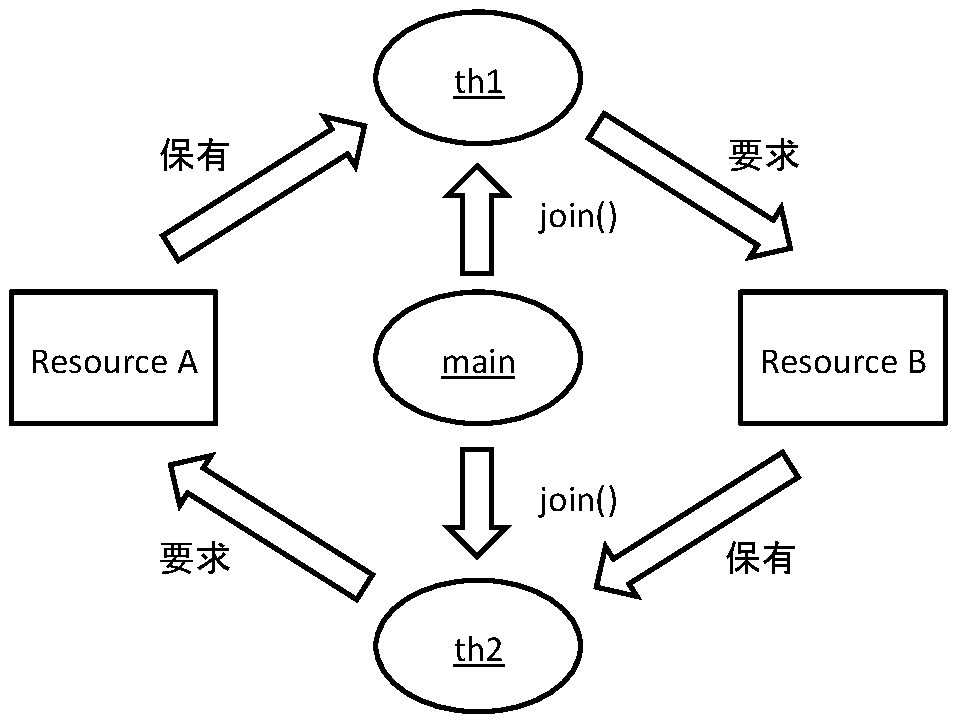
\includegraphics[width=11cm]{images/deadlock-search.pdf}
\caption{デッドロックのモデル化}
\label{figure:deadlock-search}
\end{figure}

th1 と th2 で循環鎖が形成され,デッドロック成立条件として最後に残っていた循環待ち条件が満たされ,デッドロックに陥った事が確認できた.

このように,JPF はデッドロックを検出するツールとしても有用であることがわかる.

\subsubsection{データ競合の検出}

データ競合は,複数のスレッドが同一の共有データへの読み書きを行い,最終状態が最後に走ったスレッドに依存する事による問題である \cite{MOS2}.スレッドのスケジューリング次第で結果が変わるこの問題は,デッドロック同様,並行処理特有の問題の一つである.

データ競合が発生するサンプルプログラムを次に示す.

\begin{lstlisting}[label=src:ex-exception, caption=データ競合の検出,language=Java]
public class Racer implements Runnable {
     int d = 42;
     public void run () {
          doSomething(1001);                   // (1)
          d = 0;                               // (2)
     }
     public static void main (String[] args){
          Racer racer = new Racer();
          Thread t = new Thread(racer);
          t.start();
          doSomething(1000);                   // (3)
          int c = 420 / racer.d;               // (4)
          System.out.println(c);
     }
     static void doSomething (int n) {
          // not very interesting..
          try { Thread.sleep(n); }
          catch (InterruptedException ix) {}
     }
}
\end{lstlisting}



地点 (4) が実行されるとき,racer.d の値には何が入っているだろうか.初期値は 2 行目にあるように 42 であるが,地点 (2) が実行されれば 0 となる.ただしこのプログラムは Thread.sleep() を用いて 1 ミリ秒差で地点 (2) が後に実行されるように仕組まれており,地点 (4) にて 420 / 20 という計算になるはずである.なお,地点 (2) が先に実行された場合は 420 / 0 となり, ArithmeticException (算術例外) が出ると考えられる.

このプログラムを JPF に掛けたときのレポートのエラー欄を抜き出したものを以下に示す.


\begin{verbatim}
====================================================== error #1
gov.nasa.jpf.listener.PreciseRaceDetector
race for field Racer@13d.d
  main at Racer.main(Racer.java:16)
		"int c = 420 / racer.d;               // (4)"  : getfield
  Thread-1 at Racer.run(Racer.java:7)
		"d = 0;                               // (2)"  : putfield
\end{verbatim}

Racer.main のスレッドと Racer.run のスレッドで共有変数 racer.d の競合状態を検出したことが端的に分かる.なお,より詳しい分析はスナップショット欄にあるが,長いので省略する.

一般的に,データ競合のデバッグは複雑化しやすい.エラーが起こる場合は,スタックトレースなどを活用して問題の発生個所を明らかにする事ができるが,データ競合の場合は結果が変わるだけでエラーにならない事も多い.

しかし JPF を用いれば,上記のようにどのスレッドとどのスレッドがどの共有データに対して競合状態になるのかを明らかにすることができるので,データ競合の問題解決において有用である.

\subsubsection{その他の機能}

JPF は,これまで挙げた各種不具合の発見のほか,設定 (プロパティ) による様々なカスタマイズ機能,実行コストなどの詳細なパフォーマンス分析,ChoiceGenerators による非決定的な状態の選択など,様々な機能が用意されている.

さらなる分析を行いたい場合のために,Listener という仕組みも用意されている.これは,JPF が状態を探索する過程でイベントを受信し,それに対応した処理を記述することで実現できる.標準の JPF では見つけられない新しい性質を検証したい場合などに有用である.

\section{アプローチ}

\subsection{JPF の問題点}

通常のソフトウェアテストでは,上から下へ状態を辿って終了状態に至ることで1つのパスとなる.一方モデル検査では,状態のマッチングを繰り返す中で,新しい状態から前の状態へバックトラックが発生する.こうしてモデル検査は,多数のテスト入力をする事なく,確実に不具合を発見することができる.

しかし,ネットワークやデータベースといった外部との入出力処理がある場合,状態探索のバックトラックにそれらが追従しない限りモデル検査が成り立たない.Java の入出力はストリームと呼ばれる概念で設計されているが,当然ながら処理の後戻り,巻き戻しといった操作は想定されていない.また実現できたとしても,膨大な入出力処理によるオーバーヘッドが探索の大きな妨げになることが考えられる.

\subsection{スタブによる解決手法}

そこで,JPF を適用する対象をアプリケーションの一部(多くの場合,業務処理など最も重要な部分)に絞り,それ以外をスタブで置き換える方式が採られる \cite{DBLP:conf/rv/Artho10}.この方式はシンプルで扱いやすく,入出力処理のオーバーヘッドもないなど多くの利点がある.

しかし,スタブによる方式には,いくつかの問題点がある.

一つ目は,スタブの作成が手作業な事である.スタブには,成功するパス,失敗するパスなど入出力で起こりうるあらゆる操作・応答が網羅されている事が求められるため,大規模複雑なソフトウェアのスタブを作るのは容易ではない.

二つ目は,スタブによって検査対象が複数になる場合に手間が増える事である.検査対象が複数のプロセスによって行われる場合,問題分析の煩雑化にも繋がる.

三つ目は,スタブの抽象度が高く,下位レイヤーに潜む問題も隠蔽される事である.抽象度が高すぎれば高すぎるほど,実際のソフトウェアの運用との隔たりが大きくなるため,十分な検査精度を保てない可能性がある.

よって,モデル検査の有用性を高めるためには,より一層の自動化を行う必要があるといえる.

\subsection{I/O キャッシュによる解決手法}

今回ネットワークアプリケーションを扱うにあたって,上記の問題を解決する事が期待されている新しい技術 ``I/O キャッシュ'' を適用する事を考えた \cite{DBLP:conf/kbse/ArthoLHTY09} .I/O キャッシュは,次のような動作原理で入出力ストリームにおける状態のバックトラックやリスタートといった操作を実現している.

\paragraph{新しい状態}

入出力ストリームをストアし,データやメッセージサイズをキャッシュする.またストリームの位置を記録する.

\begin{figure}[here]
\centering
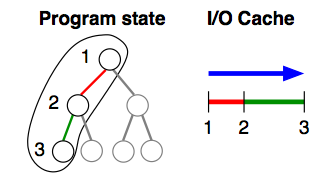
\includegraphics[width=7cm]{images/fig6a.png}
\caption{新しい状態 \cite{DBLP:conf/rv/Artho10}}
\label{figure:fig6a}
\end{figure}


\paragraph{バックトラック}

入出力状態を巻き戻す.また,ストリームの位置を前のものに変更する.

\begin{figure}[here]
\centering
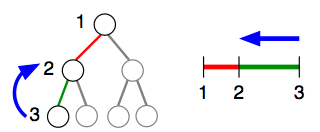
\includegraphics[width=7cm]{images/fig6b.png}
\caption{バックトラック \cite{DBLP:conf/rv/Artho10}}
\label{figure:fig6b}
\end{figure}

\newpage

\paragraph{続きの探索}

以前キャッシュされた入出力操作を再実行する.結果を確認し,もし再現できていなければエラーを出力する.

\begin{figure}[here]
\centering
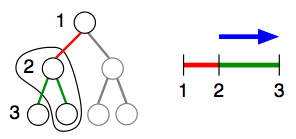
\includegraphics[width=7cm]{images/fig6c.png}
\caption{続きの探索 \cite{DBLP:conf/rv/Artho10}}
\label{figure:fig6c}
\end{figure}

\vspace{5mm}

この技術を実装したものとして ``jpf-net-iocache'' がある.これは, JPF の拡張として動作し,java.io パッケージに含まれる各種入出力ストリームや,java.net パッケージに含まれる Socket, ServerSocket, DatagramSocket といった通信フレームワークを検査対象にすることができる.

従って,今回は JPF と jpf-net-iocache 拡張の適用を考える.

\section{適用実験}

\subsection{適用対象}

今回適用対象に選んだのは,次のアプリケーションである.

\begin{quotation}
Javaで作るルーム機能付きチャットサーバー:CodeZine

http://codezine.jp/article/detail/193
\end{quotation}

以下,このアプリケーションを ``チャットシステム'' と呼ぶ.

チャットシステムは,サーバとクライアントの二つのプログラムから構成されており,互いに TCP/IP を介してメッセージをやりとりすることで動作する.

サーバは予め立ち上げておき,これに複数のクライアントが接続することで利用者同士のコミュニケーションを実現する.サーバでは,個々の利用者に対する処理はスレッドで行うので,複数の利用者が同時に会話することができる.またクライアントには,サーバへ操作やメッセージを送信したり,他の利用者が発した操作やメッセージを受信したりする基本的な処理のほか,部屋単位で会話を行う機能,Swing を用いたグラフィカルユーザインタフェースが備わっており,実用的なアプリケーションとなっている.
\newpage

\subsection{実験環境}

本実験を実施するにあたって用意したハードウェア環境を以下に示す.

\begin{table}[here]
\caption[ハードウェア環境]{ハードウェア環境}
\label{table:hardware-env}
\begin{center}
\begin{tabular}{ll}
\toprule
項目 & 内容 \\
\midrule
パソコン & Acer Aspire 1830 \\
CPU & Intel Pentium U5400 (1.2GHz Dual-Core) \\
RAM & 4GB DDR3 \\
ストレージ & 160GB HDD \\
\bottomrule
\end{tabular}
\end{center}
\end{table}

また,ソフトウェア環境は以下の通りである.

\begin{table}[here]
\caption[ソフトウェア環境]{ソフトウェア環境}
\label{table:software-env}
\begin{center}
\begin{tabular}{ll}
\toprule
項目 & 内容 \\
\midrule
オペレーティングシステム & Debian GNU/Linux 7 ``wheezy'' (testing) \\
JRE, JDK & OpenJDK 1.7 (IcedTea) \\
jpf-core & v6.0 (rev 650) \\
jpf-net-iocache & rev 42 \\
\bottomrule
\end{tabular}
\end{center}
\end{table}

なお,jpf-core および jpf-net-iocache は Mercurial レポジトリ \footnote{http://babelfish.arc.nasa.gov/hg/jpf/jpf-core} \footnote{http://babelfish.arc.nasa.gov/hg/jpf/jpf-net-iocache} より取得し,手元で ant によるビルドを行ったものを利用した.

\subsection{適用手順}

\subsubsection{適用方針}

チャットシステムのサーバプログラムとクライアントプログラムは,その処理内容に注目すると次の3種類に大別できる.

\newpage

\begin{itemize}
\item 基本処理: ユーザ管理,部屋管理,イベント処理など
\item 通信処理: 通信確立,メッセージ・コマンド送受信
\item 画面処理: メッセージ表示,操作受付など
\end{itemize}

これらのうち,画面処理に関してはチャットシステム全体の動作において必須ではなく,また GUI を JPF 単体で検査することはできない為 \footnote{JPF の拡張に jpf-awt があり,これを用いればユーザ入力に応じたモデル検査を行う事ができる.},今回は検査対象から除外する事とした.

\subsubsection{クライアントプログラムの改変}

最初に,画面処理の分離を行う.

クライアントプログラムのソースコードを調べると,画面処理は,sendMessage() メソッドを呼び出すことで基本処理にアクセスしている事がわかった.これは,ボタンを押下した際の処理を記述した部分に現れている.

\begin{lstlisting}[label=src:client-event, caption=クライアントプログラムのイベントハンドラ,language=Java]
    //ボタンが押されたときのイベント処理
        public void actionPerformed(ActionEvent e) {
            String cmd = e.getActionCommand();
            if(cmd.equals("submit")) {	//送信
                sendMessage("msg " + msgTextField.getText());
                msgTextField.setText("");
            }
            else if(cmd.equals("rename")) {	//名前の変更
                sendMessage("setName " + nameTextField.getText());
            }
            else if(cmd.equals("addRoom")) {	//部屋を作成
                String roomName = nameTextField.getText();
                sendMessage("addRoom " + roomName);
            (以下略)
\end{lstlisting}

イベントハンドラから呼び出されている sendMessage() 呼出しをまとめると,以下の 6 種類となった.

\newpage

\begin{itemize}
\item sendMessage("msg メッセージ") : 所属している部屋に対してメッセージを送信する操作
\item sendMessage("setName 名前") : 名前を変更する操作
\item sendMessage("addRoom 部屋名") : 新しい部屋を追加する操作
\item sendMessage("getUsers 部屋名") : 所属している部屋の利用者一覧を取得する操作
\item sendMessage("enterRoom 部屋名") : 指定した部屋名の部屋へ入る操作
\item sendMessage("exitRoom 部屋名") : 指定した部屋から抜ける操作
\end{itemize}

つまり,利用者が行う操作はこれらの何れか,または接続・切断処理だけとなる.これが分かったところで,クライアントプログラムから GUI 依存部分 (java.awt, javax.swing パッケージのクラスを参照する部分) を全て削除し,画面処理の切り離しを完了させた.

次に,利用者が入力する可能性がある全ての操作を網羅するために,JPF の機能である ChoiceGenerators を用いたイベント生成処理を記述した.ChoiceGenerators は,モデル検査において非決定的な状態遷移を再現したい場合に用いられる.boolean (真偽値),int (整数),double (倍精度浮動小数点数) といった値を生成するメソッドが JPF Verify API に含まれており,今回使用した getInt は,第 1 引数を開始値,第 2 引数を終了値とした数値集合分のパスを試行することができる.これを適用した様子が次のソースコードである.

\begin{lstlisting}[label=src:event-gen, caption=クライアントプログラムのイベント生成処理,language=Java]
    int maxTry = 7;
    for (int i = 0; i <= maxTry; i++) {
        int operation = Verify.getInt(0, 7);    // C/G
        switch (operation) {
        case 0:	sendMessage("getRooms");		break;
        case 1:	sendMessage("setName " + "User" + id);	break;
        case 2:	sendMessage("addRoom " + room);		break;
        case 3:	sendMessage("enterRoom " + room);	break;
        case 4:	sendMessage("msg " + "TestMessage");	break;
        case 5:	sendMessage("exitRoom " + room);	break;
        case 6:	sendMessage("DUMMY_MESSAGE");		break;
        case 7: sendMessage(null);			break;
        }
    }
\end{lstlisting}

ここでは,GUI を調査して得られた 6 つの操作に加えて,仕様にないダミーメッセージや,空のメッセージなど,想定外の入力も考慮した検証を行う事にした.

\subsubsection{サーバプログラムの改変}

チャットサーバはもちろん大多数のクライアントサーバシステムは,1つのサーバに複数のクライアントが接続し,同時にサービスを受ける.つまり,サーバとクライアントは ``1対多'' の関係にあるといえる.では,1対多の関係に対して状態の探索を始めた場合,状態数はどうなるだろうか.実際に試したところ,JPF は永遠と接続するクライアント数を増やして新たな状態を生成し続けた.

よって,結果を得るためには接続できるクライアント数を有限にする必要がある.また,制限するクライアント数によって状態数も大きく変わる事が考えられるので,接続クライアント数 (最大同時接続数) を 1 台から 2 台,3 台と変更しながら検査するために,サーバの接続待受け処理の部分に以下のような改変を施した.

\begin{lstlisting}[label=src:server-loop, caption=サーバプログラムの接続制御,language=Java]
    //main メソッドから呼び出される
    public void start(int userLimit) {    // 引数を追加
        try {
            boolean connected = false;
            server = new ServerSocket(2815);
            
            //while(!server.isClosed()) {    // コメントアウト
            for (int i = 0; i < userLimit; i++) {    // 追加
                //新しいクライアントの接続を待つ
                Socket client = server.accept();

                //ユーザーオブジェクトを生成する
                ChatClientUser user = new ChatClientUser(client);
                addUser(user);
            }
            System.exit(0);    // 追加
        } catch(IOException err) {
            err.printStackTrace();
        }
    }
\end{lstlisting}

main() メソッドでプログラム引数を受け取り,.jpf ファイルから最大同時接続数を指定できるように変更した.そしてその数を上記 start() メソッドに渡し,その分だけ ServerSocket の accept() メソッドが動作するようループ条件を改変した.以上により,無制限だった接続数を有限に抑えることができた.

\subsection{実験内容と結果}

実験は,サーバ側の引数(最大同時接続数)を 1,2,3,4 と増加させて実行し,それぞれの出力結果,実行時間や状態数の変化,そして I/O キャッシュのヒット率を中心に観察した.

\subsubsection{出力結果}

最大同時接続数 1〜3 の場合は,「no errors detected」と表示され,エラーは検出されなかった.

しかし,最大同時接続数 4 の場合は,実行開始から 11 時間 34 分を過ぎたところで OutOfMemoryError によって異常終了した.これは,Java 仮想マシンのヒープ領域が不足した場合に起きる現象で,実験の場合は 1GB を使い切っていた.

\subsubsection{実行時間及び状態数の変化}

最大同時接続数 1〜3 の場合の分析結果を以下の表に示す.

\begin{table}[here]
\caption[同時接続数 1〜3 の実験結果]{同時接続数 1〜3 の実験結果}
\label{table:result-stat}
\begin{center}
\begin{tabular}{crrc}
\toprule
同時接続数 & 実行時間 & 総和 & (new, visited, backtracked, end)  \\
\midrule
1 & 1 秒 &  {\bf 114} & (32, 19, 50, 13)  \\
2 & 10 秒 &  {\bf 29247} & (4629, 9168, 13796, 1654)  \\
3 & 35 分 54 秒 &  {\bf 9504643} & (1141855, 3419272, 4561126, 382390)  \\
\bottomrule
\end{tabular}
\end{center}
\end{table}

同時接続数を増やすに従って,実行時間や状態数が著しく増加し,組合わせ爆発が起きているといえる.

同時接続数を X 軸に,各種状態数を Y 軸にとった片対数グラフにこれらの数値をプロットすると,図 \ref{figure:graph2} のようになった.

\newpage

\begin{figure}[here]
\centering
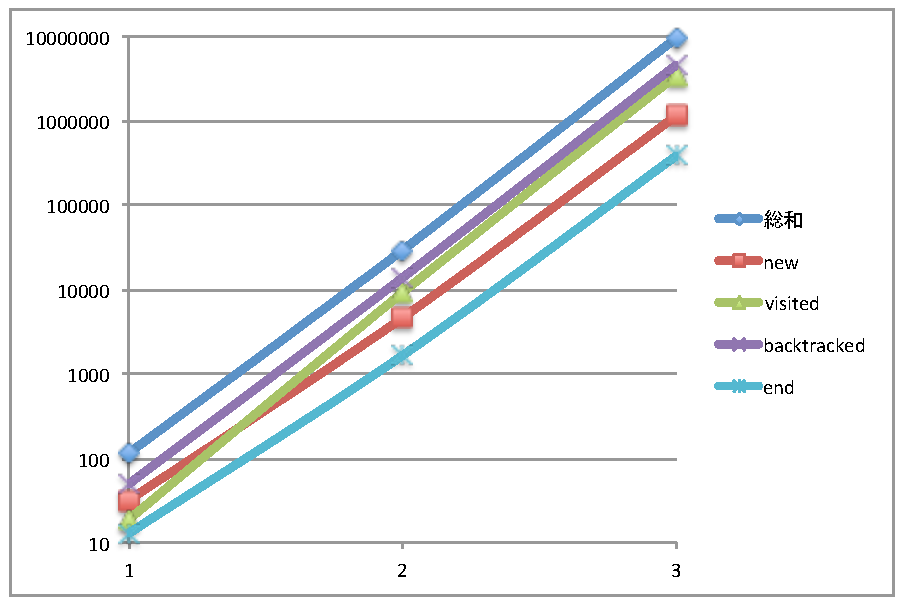
\includegraphics[width=12cm]{images/graph2.pdf}
\caption{同時接続数と各種状態数の関係}
\label{figure:graph2}
\end{figure}

見ると,各近似線はほぼ直線になっており,この事から各状態の数は指数関数的増加をしているといえる.同時接続数 1 の時のみ new 状態数が比較的多いのは,何もない状態から探索木を開拓している為と考えられる.visited 状態数が逆に少ないのも同様の理由からと推測される.

\subsubsection{I/O キャッシュにおけるヒット率}

net-iocache の結果としてキャッシュのヒット数,ミス数も計測できたので,その結果を以下の表に示す.ヒット率はヒット数,ミス数より算出した.

\begin{table}[here]
\caption[同時接続数 1〜3 のキャッシュヒット率]{同時接続数 1〜3 のキャッシュヒット率}
\label{table:result-cache}
\begin{center}
\begin{tabular}{crrr}
\toprule
同時接続数 & HIT & MISS & \% \\
\midrule
1 & 0 & 177 & 0\% \\
2 & 3207 & 280 & 91.97\% \\
3 & 935685 & 455 & 99.95\% \\
\bottomrule
\end{tabular}
\end{center}
\end{table}

当然ながら,これらの数値は入出力操作の回数と関係している.同時接続数 1 のときにキャッシュのヒットが皆無なのは,全てが新しい入出力操作だからである.

また,キャッシュミス数をグラフにしたものが図 \ref{figure:graph3} である.

\newpage


\begin{figure}[here]
\centering
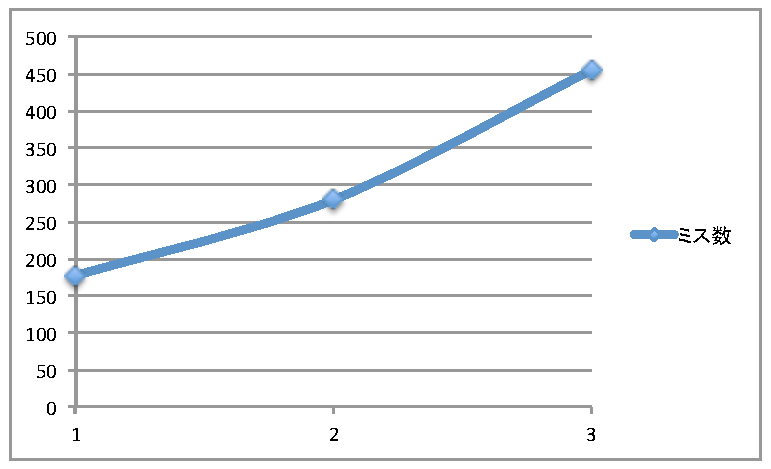
\includegraphics[width=12cm]{images/graph3.pdf}
\caption{同時接続数と実行時間の関係}
\label{figure:graph3}
\end{figure}

ミス数の増加具合はほぼ一定に増加している.つまり,キャッシュミスする入出力操作(新たな入出力操作)は,接続されるクライアントの分だけ増えるという事を意味している.一方で全体の入出力操作数は状態数と同じく指数関数的に増大しているので,キャッシュはパフォーマンスの上でも大きな役割を果たしている事がわかる.

\section{考察}

\subsection{JPF 及び net-iocache の有用性について}

今回の実験では,JPF 及び net-iocache は期待通りに動作し,適用のための改変を行ったチャットシステムに対しエラーなしという結果を得た.これによって,一般的なネットワークアプリケーションに対しても JPF を適用できることを示すことができた.

また,I/O キャッシュによる手法を用いたことで,(サーバ・クライアントそれぞれに I/O スタブの実装や検査プロセスを行う必要がある)スタブによる手法と比べ,より JPF による自動化の割合を増やし,また単一の検査プロセスで結果が得られるようになった.これにより,I/O キャッシュの有用性を示すことができたといえる.

\subsection{適用対象の分析結果について}

今回の適用対象に対する結果からは,次の 3 点が言える.

\begin{enumerate}
\item ハンドルされない例外やエラーはなかった
\item デッドロックは検出されなかった
\item データ競合は検出されなかった
\end{enumerate}

1 つ目に関しては,Java の例外処理においてスローされる可能性のある全ての例外がプログラム自身で想定されている事を示せた事になる.なお,よく見落とされがちな例外として,空のオブジェクトを参照してしまう NullPointerException や,ゼロ除算などで発生する ArithmeticException,配列外のインデックス番号を参照してしまう IndexOutOfBoundsException などが挙げられる.

2 つ目に関しては,デッドロックによってチャットシステムの動作が停止してしまう事がないことを示せたことになる.デッドロックは,相互排除性,保有と待ち条件,横取りなし条件,循環待ち条件といった性質が重なった場合に発生するが,この問題の分析や解決は困難を極めることが多い \cite{MOS2}.モデル検査によって発生しない事が示されている事は高信頼化に大きく貢献する.

3 つ目に関しては,スレッドのスケジュール順によって共有データの更新などの処理が期待通りに動かないといった問題がないことを示せたことになる.データ競合は,簡単なテストでは見つからない事も少なくないため,モデル検査で競合が起きない事が示される事には価値がある.

\subsection{組合わせ爆発の問題について}

今回,最大同時接続数を 3 より大きくすることができなかった.また 3 の場合でも数十分単位で時間が掛かっており,非力なノートパソコンで試したとはいえあまりにも時間が掛かっている.

実験結果から,同時接続数が増えるほど状態数が指数関数的に増加することが明らかになった.チャットシステムのサーバプログラムでは,クライアントの数だけスレッドが生成され,別々のクライアントの対話は別々のスレッドが行っている.つまり,スレッドの並列度と状態数が密接に関わっていると言える.状態数を抑えるには,並列度を必要最小限度にするなどの工夫が必要と考えられる.

また,ChoiceGenerators も状態数を増やす原因の一つである.これも,むやみに適用するのではなく,必要なところに必要なだけ用いるようにして状態数を抑える必要があるだろう.

そして,どうしても組合わせ爆発を解決できない場合には,検査対象をより限定する必要がある.適度な規模のソフトウェアへ,適切にツールを適用してく事が,モデル検査を効率よく現実のプログラムに適用していくためには欠かせないと言える.

\newpage

\subsection{より高度な検査について}

本レポートでは,JPF 及び net-iocache の適用方法を中心に扱ったが,実際に何らかのアプリケーションに対して今回の方法で適用するだけでは充分なソフトウェア検証とはいえない.ソフトウェアの正しさを証明するためには,仕様を満たしているかを一つ一つ確認する事が大前提であり,JPF はそのために様々な手段を提供している.

最も典型的な方法は,アサーション (表明) の挿入である.アサーションを用いてシステムの仕様をプログラム中に記述できれば,JPF に備わっているハンドルされない例外・エラー検出機能で容易にアサーション違反を発見することができる.

今回の実験でも,いくつか思いついたアサーションを数個挿入して簡単な検査も実施したが,問題なくパスすることができた.実際の検証プロセスでは,アプリケーションの利用環境などに応じて適切な仕様を策定し,必要なアサーションを綿密に定義し挿入していく事が望ましいのは言うまでもない.

\section{まとめ}

JPF は,Java バイトコードを対象にした優れたソフトウェアモデル検査器であり,プログラムを解析し状態を抽出,それらを網羅的に探索することで仕様の確認や不具合の発見を効率よく行うことができる.一方で,その動作原理ゆえに様々な制約があり,適用できる対象は限られていた.

しかし,JPF に関する調査を重ねるうちに,一般的なアプリケーションに対しても,適用個所を限定したり,拡張ツールを組み合わせたりすることで JPF の機能を活用することができることが分かった.そこで本レポートは,チャットシステムを題材にして,JPF とその拡張の net-iocache を適用するための方法を研究し,実際に適用してモデル検査を実行できることを示した.

実際のアプリケーションにこうしたモデル検査を少ないコストで適用できる事は,手作業が随所に入る手間のかかるテスト技法よりも,経済的側面,時間的側面,そして正確性について優位になる事を意味する.現状では,本レポートでも取りあげた組合わせ爆発問題など,まだまだ解決・改善すべき課題は少なくないが,大規模複雑化が進む今日のソフトウェア業界にとって,潜在的なニーズがある技術とも言える.

将来性のある最先端の技術としてこれからも動向に注視してゆきたい.



\section{謝辞}

本研究を実施するにあたり,副テーマ指導教官の青木利晃准教授より,丁寧かつ熱心なご指導を賜りました.ここに感謝の意を表します.

\bibliographystyle{jplain}
\bibliography{MinorResearchReport}

\end{document}